% Task 2
\documentclass[12pt,a4paper,english]{extarticle}
\usepackage[T1]{fontenc}
\usepackage[utf8]{inputenc}
\usepackage{fourier}
\usepackage{geometry}
\geometry{verbose,tmargin=2.2cm,bmargin=2cm,lmargin=2.2cm,rmargin=2cm}
\usepackage{float}
\usepackage{textcomp}
\usepackage{amsmath}
\usepackage{stackrel}
\usepackage{graphicx}
\usepackage{esint}
\usepackage{tikz}
\usepackage{array}
\usepackage{multirow}
\usetikzlibrary{matrix,calc}

\makeatletter

\providecommand{\tabularnewline}{\\}

\usepackage{fancyhdr}
\usepackage{lscape}
\usepackage{amssymb}
\pagestyle{fancy}
\lhead{Electronica III - 22.13}
\chead{TPL3}
\rhead{ITBA}
\renewcommand{\headrulewidth}{1pt}
\renewcommand{\footrulewidth}{1pt}

\makeatother

\usepackage[english]{babel}

\begin{document}

\section*{Task 2}

In this section, the objetive is to recognize a 
sequence of 4 bits that come in a synchronized
way. If the sequence is recognized, an output 
is turned on. Using a Moore's state machine,
the resulting diagram is as shown below.

\begin{figure}[H]
    \begin{centering}
    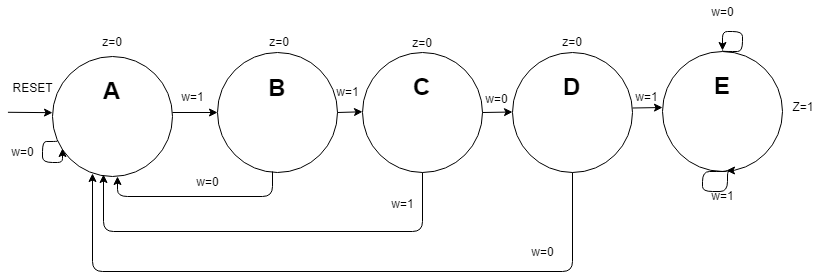
\includegraphics[width=0.8\textwidth]{Graficos2/2a_fsm.png}
    \par\end{centering}
    \caption{Moore state machine diagram}
\end{figure}

Notice that when the sequence is recognized, 
the machine needs to be reseted to detect a 
new combination. With the diagram, the following transition table 
is made.

\begin{figure}[H]
    \begin{centering}
\begin{tabular}{|c|c|c|c||c|}
    \hline 
    \multicolumn{2}{|c|}{Estado Actual} & \multicolumn{2}{c||}{Estado Siguiente} & \multicolumn{1}{c|}{Salidas}\tabularnewline
    \hline 
    \hline 
    \multirow{2}{*}{} & \multirow{2}{*}{y3 - y2 - y1} & \multicolumn{2}{c||}{W} & \multirow{2}{*}{Z}\tabularnewline
    \cline{3-4} 
     &  & \multicolumn{1}{c|}{0} & \multicolumn{1}{c||}{1} & \tabularnewline
    \hline 
    A & 000 & A & B & 0\tabularnewline
    \hline 
    B & 001 & A & C & 0\tabularnewline
    \hline 
    C & 010 & D & A & 0\tabularnewline
    \hline 
    D & 011 & A & E & 0\tabularnewline
    \hline 
    E & 100 & E & E & 1\tabularnewline
    \hline 
    \end{tabular}
    \caption{Moore state machine - Transitions}
\end{centering}
\end{figure}

Using Karnaugh's maps (see resolution in $Annex$), the functions for
the diferent states and the output are made
as follows: $Y_3 = y_3 + y_2 \cdot y_1 \cdot W$, $Y_2 = y_2 \cdot \overline{y_1} \cdot \overline{W} + \overline{y_2} \cdot y_1 \cdot W$,
and $Y_1 = \overline{y_3} \cdot \overline{y_2} \cdot \overline{y_1} \cdot W + y_2 \cdot \overline{y_1} \cdot \overline{W}$.
Frome the table of transitions, $Z = y_3$.
\newpage
With the functions, the state machine is 
implemented using three D Flip Flops as shown below.

\begin{figure}[H]
    \begin{centering}
    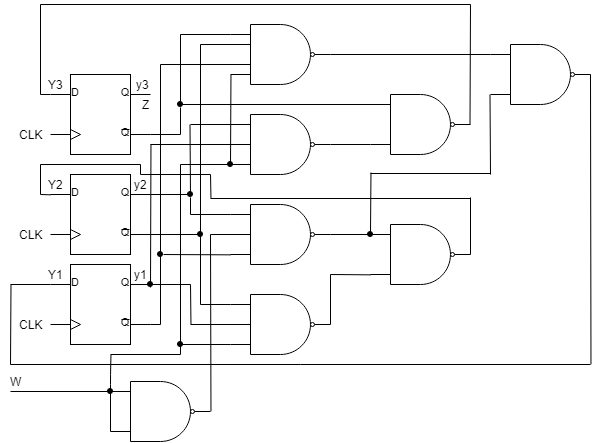
\includegraphics[width=0.8\textwidth]{Graficos2/2a_Compuertas_Moore.png}
    \par\end{centering}
    \caption{Moore state machine  - Circuit implementation}
\end{figure}

Now, the same system is implemented using a Mealy's 
state machine, wich resulting diagram is shown below.

\begin{figure}[H]
    \begin{centering}
    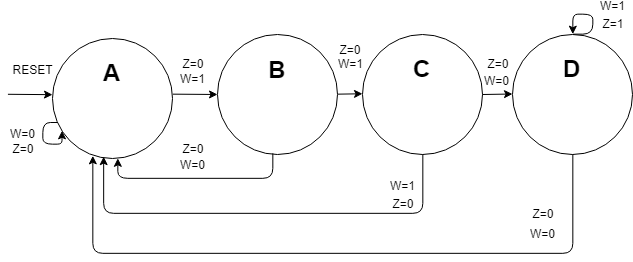
\includegraphics[width=0.8\textwidth]{Graficos2/2b_fsm.png}
    \par\end{centering}
    \caption{Mealy state machine diagram}
\end{figure}
\newpage
Using the diagram, a table with the state 
transitions is made.
\begin{figure}[H]
    \begin{center}
\begin{tabular}{|c|c|c|c||c|c|}
    \hline 
    \multicolumn{2}{|c|}{Estado Actual} & \multicolumn{2}{c||}{Estado Siguiente} & \multicolumn{2}{c|}{Salidas}\tabularnewline
    \hline 
    \hline 
    \multirow{2}{*}{} & \multirow{2}{*}{y2 - y1} & \multicolumn{2}{c||}{W} & \multicolumn{2}{c|}{Z}\tabularnewline
    \cline{3-6} 
     &  & \multicolumn{1}{c|}{0} & \multicolumn{1}{c||}{1} & W=0 & W=1\tabularnewline
    \hline 
    A & 00 & A & B & 0 & 0\tabularnewline
    \hline 
    B & 01 & A & C & 0 & 0\tabularnewline
    \hline 
    C & 10 & D & A & 0 & 0\tabularnewline
    \hline 
    D & 11 & A & D & 0 & 1\tabularnewline
    \hline 
    \end{tabular}
    \caption{Mealy state machine - Transitions}
\end{center}
\end{figure}

Using Karnaugh's maps (see resolution in $Annex$), the functions for the 
states and the output are as follows: $Y_2 = W \cdot y_1 + \overline{W} \cdot y_2 \cdot \overline{y_1}$, $Y_1 = W \cdot \overline{y_2} \cdot \overline{y_1} + W \cdot y_2 \cdot y_1 + \overline{W} \cdot y_2 \cdot \overline{y_1}$, 
and $Z = W \cdot y_2 \cdot y_1$.
With the defined functions, the state machine 
is implemented with 2 D Flip Flops. In this case
is used one less flip flop, and the machine can
used again without reset it.

\begin{figure}[H]
    \begin{centering}
    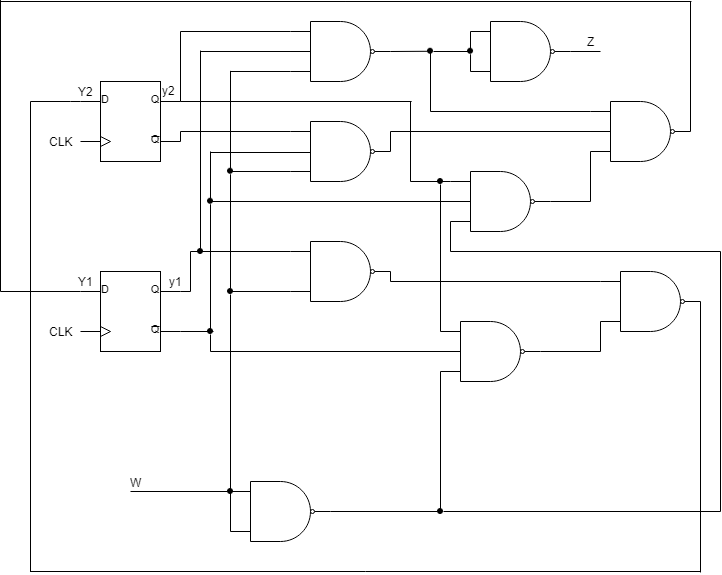
\includegraphics[width=0.8\textwidth]{Graficos2/2b_Compuertas_Mealy.png}
    \par\end{centering}
    \caption{Mealy state machine - Circuit implementation}
\end{figure}

\end{document}